%%%%%%%%%%%%%%%%%%%%%%%%%%%%%%%%%%%%
% This is root file of the thesis. %
%%%%%%%%%%%%%%%%%%%%%%%%%%%%%%%%%%%%

%\documentclass[11pt,a4paper,oneside]{thesis}
\documentclass[11pt,a4paper,]{thesis}
\usepackage{amssymb}
\usepackage{amsbsy}
\usepackage{amsmath}
\usepackage{amsthm} % This is only for theorem and proofs.
\usepackage{setspace}
\usepackage{ifpdf}
\ifpdf
\usepackage[pdftex]{graphicx}
\else
\usepackage{graphicx}
\fi
\usepackage{cite}

\usepackage[pdfpagemode={UseOutlines},bookmarks=true,bookmarksopen=true,
bookmarksopenlevel=0,bookmarksnumbered=true,hypertexnames=false,
colorlinks,linkcolor={blue},citecolor={blue},urlcolor={blue},
pdfstartview={FitV},unicode,breaklinks=true]{hyperref}

\title{Lightening the Load: A New Playback Engine for Sophisticated Animated Lighting Displays}
\author{\href{yz4116@imperial.ac.uk}{Yubo~Zhi}\\
Project supervisor: \href{james.davis06@imperial.ac.uk}{Dr~James~J.~Davis}}


%%%%%%%%%%%%%%%%%%%%%%%%%%%%%%%%%%%%
% including page setting & fancyhdr.
\setlength{\textwidth}{500pt}
\addtolength{\hoffset}{-20pt}
\setlength{\textheight}{650pt}
\setlength{\headsep}{30pt}

% Set left margin - The default is 1 inch.
\setlength{\oddsidemargin}{2cm}

% Set width of the text - What is left will be the right margin.
\setlength{\textwidth}{15cm} %5.7in

% Set top margin - The default is 1 inch
\setlength{\topmargin}{-1.5cm}

% Set height of the header
\setlength{\headheight}{1.2cm}

% Set vertical distance between the header and the text
\setlength{\headsep}{1.2cm}

% Set height of the text
\setlength{\textheight}{23cm} %9in

% Set vertical distance between the text and the
% bottom of footer
\setlength{\footskip}{0.4cm}

% set belowcaptionskip.
\addtolength{\belowcaptionskip}{2ex}

%\setlength{\parindent}{2em}
\setlength{\parindent}{0pt}
%%%%%%%%%%%%%%%%%%%%%
\usepackage{fancyhdr}

\pagestyle{fancy}

\renewcommand{\chaptermark}[1]{\markright{\thechapter.\ #1}}
\renewcommand{\sectionmark}[1]{\markright{\thesection\ #1}}
\fancyhf{}
\fancyhead[LE,RO]{\bfseries\thepage}
\fancyhead[LO]{\bfseries\rightmark}
\fancyhead[RE]{\bfseries\leftmark}
\renewcommand{\headrulewidth}{0.5pt}
\renewcommand{\footrulewidth}{0pt}
\addtolength{\headheight}{0.5pt}
\fancypagestyle{plain}{
  \fancyhead[LE,RO]{\bfseries\thepage}
  \fancyhead[LO]{}
  \fancyhead[RE]{}
  \renewcommand{\headrulewidth}{0.5pt}
}

\def\mystretch{1.5}

\newlength{\figX}
\newlength{\figY}
\newlength{\tmplen}

\newlength{\matFigX}
\newlength{\matFigY}

\setlength{\matFigX}{4.04in} \setlength{\matFigY}{3.04in}

\setlength{\parindent}{0pt}
\setlength{\parskip}{1ex}
%\setlength{\parindent}{3em}
\sloppy

\hyphenation{another}

%%%%%%%%%%%%%%%%%%%%%%%%%%%%%%%%%%%
\usepackage[caption=false,font=footnotesize]{subfig}
\usepackage[pdftex,dvipsnames]{xcolor}
\usepackage{listings,xargs,epsfig,enumitem}
\usepackage[colorinlistoftodos,prependcaption,textsize=small]{todonotes}

\graphicspath{{Figs/}}

\definecolor{dkgreen}{rgb}{0,0.6,0}
\definecolor{gray}{rgb}{0.5,0.5,0.5}
\definecolor{mauve}{rgb}{0.58,0,0.82}
\newcommand{\fsize}{\small}
%\newcommand{\fsize}{\tiny}
\newcommand{\tabsize}{4}

\lstset{frame=tb,
  language=C++,
  %  aboveskip=0mm,
  belowskip=0mm,
  showstringspaces=false,
  columns=flexible,
  basicstyle={\fsize\ttfamily},
  numberstyle=\fsize\color{gray},
  %  numbers=left,
  keywordstyle=\color{blue},
  commentstyle=\color{dkgreen},
  stringstyle=\color{mauve},
  breaklines=true,
  breakatwhitespace=true,
  tabsize=\tabsize
}

\graphicspath{{Figs/}}

% Hyper references
\newcommand{\fref}[1]{Fig.~\ref{#1}}
\newcommand{\eref}[1]{(\ref{#1})}
\newcommand{\tref}[1]{\tablename~\ref{#1}}
\newcommand{\lref}[1]{Listing~\ref{#1}}
\newcommand{\cref}[1]{Chapter~\ref{#1}}
\newcommand{\aref}[1]{Appendix~\ref{#1}}
\newcommand{\sref}[1]{Section~\ref{#1}}

% Colours
\definecolor{dkgreen}{rgb}{0,0.6,0}
\definecolor{mauve}{rgb}{0.58,0,0.82}
\definecolor{gray}{rgb}{0.4,0.4,0.4}
\definecolor{darkblue}{rgb}{0.0,0.0,0.6}
\definecolor{cyan}{rgb}{0.0,0.6,0.6}
\definecolor{darkorange}{rgb}{0.8,0.4,0.0}

% Coloured text
\newcommand{\wn}[1]{{\color{cyan}#1}}

\newcommand{\ca}[1]{{\color{darkorange}#1}}
\newcommand{\cad}[1]{{\color{darkorange}\sout{#1}}}

\renewcommand{\ca}[1]{#1}
\renewcommand{\cad}[1]{}
\newcommand{\cb}[1]{{\color{darkorange}#1}}

\renewcommand{\cb}[1]{#1}
\newcommand{\cc}[1]{{\color{darkorange}#1}}
\newcommand{\ccd}[1]{{\color{darkorange}\sout{#1}}}
\newcommand{\cmtc}[1]{\cmt{#1}}

\renewcommand{\cc}[1]{#1}
\renewcommand{\ccd}[1]{}
\renewcommand{\cmtc}[1]{}

% Todo boxes
\newcommandx{\improv}[2][1=]{\todo[linecolor=Plum,backgroundcolor=Plum!25,bordercolor=Plum,#1]{#2}}
\newcommand{\cmt}[1]{\improv[inline]{#1}}

% Code listing
\newfloat{lstfloat}{htbp}{lop}

\newcommand{\fsize}{\small}
%\newcommand{\fsize}{\tiny}
\newcommand{\tabsize}{8}

\lstdefinelanguage{XML}
{
  morestring=[b]",
  morestring=[s]{>}{<},
  morecomment=[s]{<?}{?>},
  stringstyle=\color{black},
  identifierstyle=\color{darkblue},
  keywordstyle=\color{cyan},
  morekeywords={xmlns,version,type}% list your attributes here
}

\lstset{frame=tb,
  language=C++,
  %  aboveskip=0mm,
  belowskip=0mm,
  showstringspaces=false,
  columns=flexible,
  basicstyle={\fsize\ttfamily},
  numberstyle=\fsize\color{gray},
  %  numbers=left,
  keywordstyle=\color{blue},
  commentstyle=\color{dkgreen},
  stringstyle=\color{mauve},
  breaklines=true,
  breakatwhitespace=true,
  tabsize=\tabsize
}


%%%%%%%%%%%%%%%%%%%%%%%%%%%%%%%%%%%
% The Beginning of a LaTeX document
\begin{document}

%%%%%%%%%%%%%%%%%%%%%%%%%%%%%%%%
% The Cover Page of PhD Thesis %
%%%%%%%%%%%%%%%%%%%%%%%%%%%%%%%%
\thispagestyle{empty}

\begin{center}
\null \vspace{\stretch{0.2}}
\renewcommand{\baselinestretch}{2}

\begin{textblock*}{7cm}(17.5mm, 17.5mm)%
  
\epsfig{file=ic.eps,width=7cm,clip=}%
\end{textblock*}

{\huge \textsc{Lightening the Load: A New Playback Engine for Sophisticated Animated Lighting Displays} \par}
\vspace{\stretch{1}}

\textsc{\large\href{yz4116@imperial.ac.uk}{Yubo~Zhi}} \\
\textit{B.Eng}(\textit{Hons})\\
\vspace{\stretch{1}}
\ca{\large Project supervisor: \href{james.davis06@imperial.ac.uk}{Dr~James~J.~Davis}}
\vspace{\stretch{0.1}}

A \ca{dissertation} submitted in fulfilment of requirements for the degree of \\
Master of Science\\
Analogue and Digital Integrated Circuit Design\\
of Imperial College London

\vspace{\stretch{1}}
%\centerline{\special{bmp:ic.bmp x=2cm}}

Department of Electrical and Electronic Engineering\\
Imperial College London\\
\today

\end{center}


%%%%%%%%%%%%%
\frontmatter
\doublespace
\setlength{\tmplen}{\parskip}
\setlength{\parskip}{-1ex}
\renewcommand{\baselinestretch}{1.5}
\chapter{Abstract}
\renewcommand{\baselinestretch}{\mystretch}

%\setlength{\parindent}{2em}

Vixen 3 is a fully featured, free and open-source application facilitating the design and playback of lighting sequences. It is particularly suited to the animation of holiday lighting, the variety and flexibility of which have increased dramatically in the past few years. However, as displays become more sophisticated, the original engine will need an increasing amount of processing power for real-time rendering. To resolve this problem, a new playback engine was developed in this project. This engine works based on pre-rendering the sequence to \ca{reduce} runtime computations. As a result, complex display controls are now possible on hardware platforms with relatively less processing power \ca{than desktop computers}, especially embedded devices. Together with the \ca{added} support for using video \ca{file formats as pre-rendered sequences}, this can greatly increase the flexibility, reduce the hardware requirement and cost of setting up lighting displays. \ca{For example, over 8000 \ccd{of} lighting channels can now be directly controlled from a single Raspberry Pi with stable 50 fps refresh rate, instead of requiring a computer with unstable 20 fps refresh rate.}

\renewcommand{\baselinestretch}{1.5}
\chapter{Acknowledgement}
\markright{Acknowledgement}
\renewcommand{\baselinestretch}{\mystretch}

%\setlength{\parindent}{2em}

I would like to express my sincere gratitude to my project supervisor \href{james.davis06@imperial.ac.uk}{Dr~James~J.~Davis} for supporting this project and providing invaluable comments and suggestions throughout this project.

\tableofcontents
\listoffigures
\listoftables
\renewcommand{\baselinestretch}{\mystretch}
\renewcommand{\baselinestretch}{1}
\chapter{Abbreviations}
\markright{Abbreviations}

\begin{tabular}{rl}
  \vspace{0.1em} \textbf{API:} & Application Programming Interface \\
  \vspace{0.1em} \textbf{CRF:} & Constant Rate Factor \\
  \vspace{0.1em} \textbf{CUI:} & Command-line User Interface \\
  \vspace{0.1em} \textbf{DLL:} & Dynamic-Link Library \\
  \vspace{0.1em} \textbf{fps:} & Frame per second \\
  \vspace{0.1em} \textbf{GNU:} & Recursive acronym for \ca{``}GNU's Not Unix!\ca{''}, the GNU Operating System \\
  \vspace{0.1em} \textbf{GUI:} & Graphical User Interface \\
  \vspace{0.1em} \textbf{GUID:} & Globally Unique IDentifier \\
  \vspace{0.1em} \textbf{IO:} & Input / Output \\
  \vspace{0.1em} \textbf{IoT:} & Internet-of-Things \\
  \vspace{0.1em} \textbf{JIT:} & Just-In-Time \\
  \vspace{0.1em} \textbf{LGPL:} & GNU Lesser General Public License \\
  \vspace{0.1em} \textbf{RAM:} & Random Access Memory \\
  \vspace{0.1em} \textbf{RPi:} & Raspberry Pi \\
  \vspace{0.1em} \textbf{SIMD:} & Single Instruction, Multiple Data \\
  \vspace{0.1em} \textbf{UI:} & User Interface \\
  \vspace{0.1em} \textbf{WPF:} & Windows Presentation Foundation \\
\end{tabular}


\setlength{\parskip}{\tmplen}

%%%%%%%%%%%%
\mainmatter
\fancyhead[RE]{\emph{Chapter \thechapter}}
\renewcommand{\baselinestretch}{\mystretch}
% Use \input to include your chapters as illustrated below
\chapter{Introduction}
\renewcommand{\baselinestretch}{\mystretch}
\label{chap:Intro}
%\setlength{\parindent}{0pt}

\PARstart{V}{ixen} 3 \cite{vixen} is an open-source application for designing and controlling automation lighting displays. With modern technologies, computer-controlled displays are becoming increasingly popular as holiday decorations and other lighting show projects. Vixen is capable of supporting multiple display controllers with thousands of channels for complex lighting shows and effects. It can also synchronise the lighting sequence to audio playback.

By being open-source, Vixen is primarily built towards lower cost Do-It-Yourself solutions. Together with the support of software plugins, users can create customised plugins to support a variety of display controllers, or improve the Vixen software framework itself.

However, the current execution engine used by Vixen has significant computational overheads. Consequently, a powerful computer with sufficient memory space is required to render the lighting effects in real-time. This may not be possible in some situations, increasing the cost of display setup, and is very energy inefficient.

In this project, a new engine was developed. Instead of having layers of overheads in the original execution engine, the new engine takes pre-rendered sequences exported at the display controller's layer. It was also implemented with simplicity and portability to be suitable for embedded platforms.

The concept of pre-rendering and playback performs especially similar to wildly used video processing technologies. Therefore, support for video format was also implemented for exporting and playback using the new engine. This enables users to use commonly available video editing and transcoding software on lighting sequences. Well-established video compression algorithms also help reduce data file size, potentially take advantages of hardware multimedia acceleration features. By muxing audio stream and channel information into a single video file, management and sharing of sequences were also simplified.

\chapter{Background}
\renewcommand{\baselinestretch}{\mystretch}
\label{chap:BG}
%\setlength{\parindent}{0pt}

\section{Vixen overview}

\PARstart{T}{he} Vixen application was based on Microsoft Windows .NET runtime \cite{dotnet}, developed using Microsoft Visual Studio \cite{msvs}. It is capable of loading modules as dynamic-link libraries (DLL) during runtime. Most of its components such as controllers, lighting effects and editor were implemented as separate modules. \fref{fig:vixen-main} shows the main application interface.

\begin{figure}[!t]
  \centering
  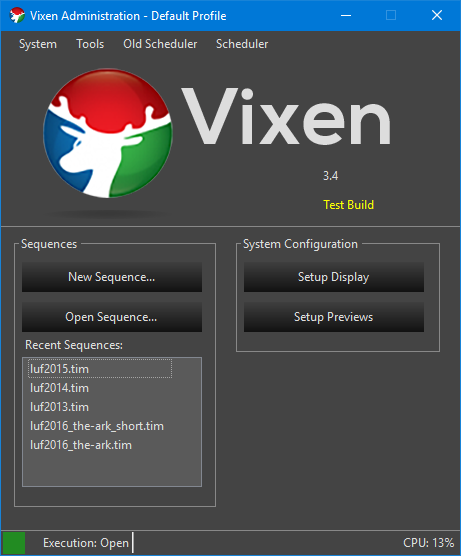
\includegraphics[width=0.6\textwidth]{Figs//vixen_main.png}
  \caption{\footnotesize Main entry GUI of Vixen application}
  \label{fig:vixen-main}
\end{figure}

The execution engine consists of 4 stages for flexible and intuitive lighting sequence editing, as shown in \fref{fig:stages}.

\begin{figure}[!t]
  \centering
  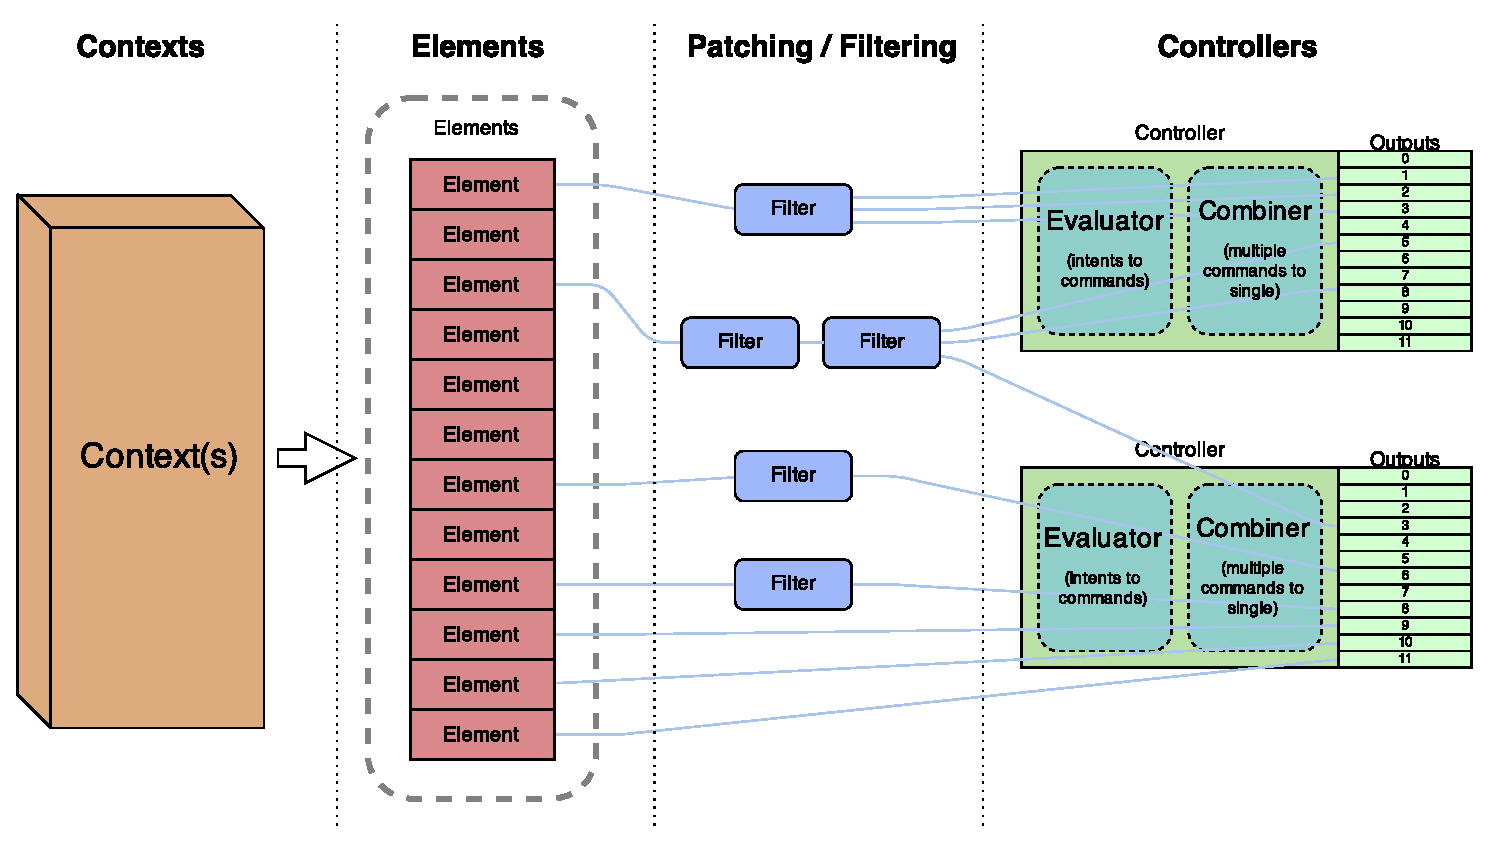
\includegraphics[width=0.85\textwidth]{Figs//V3-Engine-1.eps}
  \caption{\footnotesize Vixen execution engine stages (adopted from \cite{vixen})}
  \label{fig:stages}
\end{figure}

Contexts are at the very top level of data structures used by Vixen. Vixen stores lighting effects by sequence files, each sequence represents a context to be executed. By using a built-in show scheduler, Vixen can load, pre-render and cache multiple sequence contexts at the same time, then scheduled to be repeatedly played afterwards.

Each sequence context contains lots of elements. Elements represent abstract items described by the user. For example, lights on trees, lights on roofs, etc. They describe the visual display setup, independent of hardware controller connections. Elements can also be grouped together for management and some more advanced display effects. Vixen has a vary flexible sequence designing interface with timeline and audio support, as shown by \fref{fig:vixen-editor}.

\begin{figure}[!t]
  \centering
  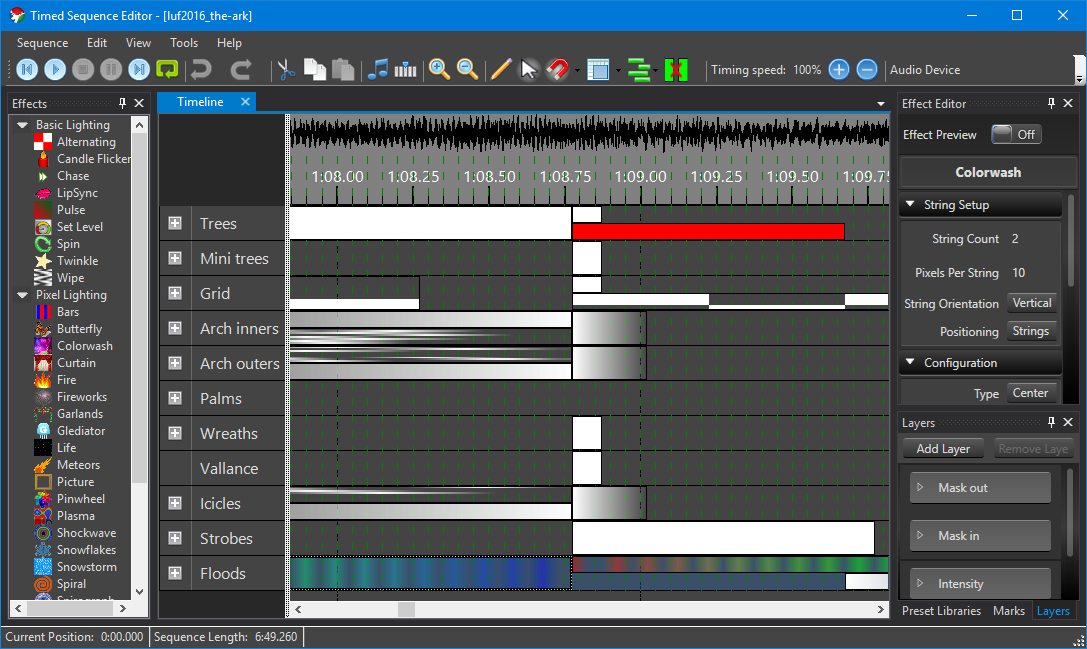
\includegraphics[width=0.9\textwidth]{Figs//vixen_editor.png}
  \caption{\footnotesize Vixen sequence editor interface}
  \label{fig:vixen-editor}
\end{figure}

Between elements and hardware controllers, filters are used to map the channel connections, and patches are used to define data linkages among them. Each element output may be discarded, duplicated or combined by the filters.

Inside each hardware controller module, data from multiple channels will be combined into a single data packet, then send through the appropriate hardware interface, which can be USB, Ethernet, etc. Each controller has its own update thread, with individual update frame rate settings.

Vixen has another dedicated configuration interface for controllers and filter connections, as shown by \fref{fig:vixen-setup}.

\begin{figure}[!t]
  \centering
  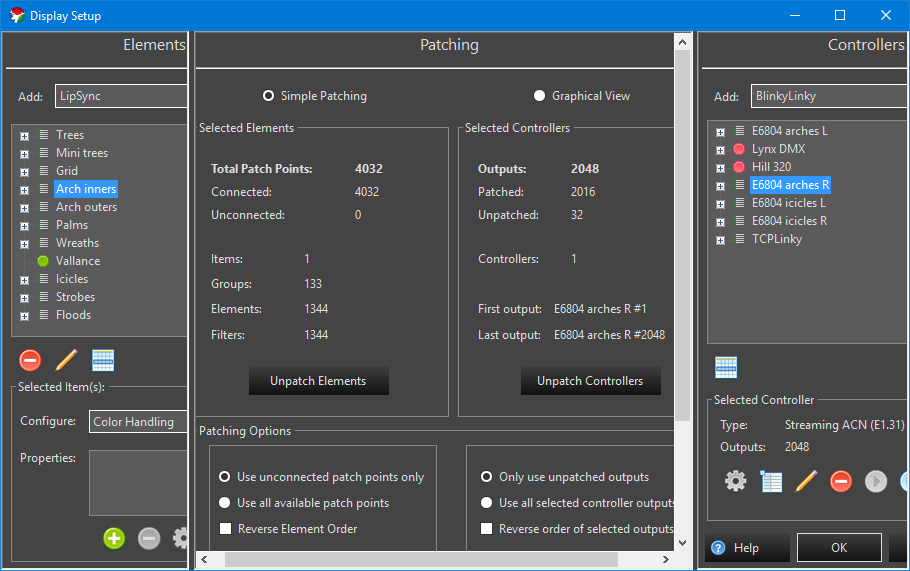
\includegraphics[width=0.9\textwidth]{Figs//vixen_setup.png}
  \caption{\footnotesize Vixen controller setup interface}
  \label{fig:vixen-setup}
\end{figure}

Vixen also has a preview display. It maps element outputs to sets of points on a 2D surface, possibly arranged as the shapes of actual physical objects. The preview was rendered on a separate window, as shown by \fref{fig:vixen-preview}.

\begin{figure}[!t]
  \centering
  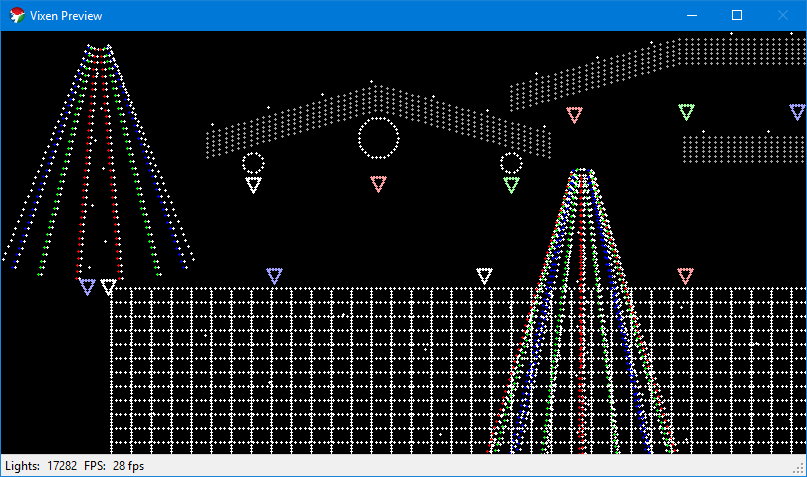
\includegraphics[width=0.9\textwidth]{Figs//vixen_preview.png}
  \caption{\footnotesize Vixen preview interface}
  \label{fig:vixen-preview}
\end{figure}

\section{Similar applications}

\cmt{Further background researches may need to be done, such as analysing other lighting control applications' performances and their implementations.}

\section{Testing platforms}

\subsection{Microsoft Windows based systems}

As the Vixen application was originally developed based on Microsoft Windows, so a mid-range laptop running Microsoft Windows 10 x64 was used as the primary development platform. It is capable of running Microsoft Visual Studio required for developing the Vixen application, but with relatively lower computation power to expose the run-time performance issue of Vixen.

This platform was also used to remotely connect to other development platforms, using technologies such as SSH.

The hardware specifications are listed below:

%\begin{enumerate}[noitemsep]
\begin{description}
  \item[CPU:]	Intel dual-core i5-3337U, 1.80 GHz
  \item[RAM:]	LPDDR3 8.0GB 1600MHz
  \item[Disk:]	Solid-state drive
\end{description}

\subsection{Linux based systems}
\label{sec:systems}

Multiple Linux based systems with a variety of resource configurations, ranging from high performance desktop platforms to low-end embedded platforms, were used for performance testing, as listed in \tref{tbl:linux}.

\begin{table}[!h]
  \centering
  \begin{tabular}{l|l|l|l|l}
    \hline
    \textbf{Name} & \textbf{Architecture} & \textbf{CPU} & \textbf{Specification} & \textbf{RAM} \\
    \hline
    NAS         & x86\_64 & AMD FX-8350       & 8 cores @ 4.0GHz  & 16GiB   \\ \hline
    Jetson TX2  & aarch64 & NVIDIA Tegra X2   & 6 cores @ 2.0GHz  & 8GiB    \\ \hline
    RPi 3B      & armv7l  & Broadcom BCM2837  & 4 cores @ 1.2GHz  & 1GiB    \\ \hline
    RPi Zero W  & armv6l  & Broadcom          & 1 core @ 1.0GHz   & 512MiB  \\ \hline
    RPi B+      & armv6l  & Broadcom BCM2835  & 1 core @ 900MHz   & 512MiB  \\ \hline
    Noah NP1380 & mipsel  & Ingenic JZ4740    & 1 core @ 336MHz   & 64MiB   \\ \hline
  \end{tabular}
  \caption{Linux based systems}
  \label{tbl:linux}
\end{table}

It is possible to install Microsoft Windows IoT system on some of the testing platforms. However, system, driver and runtime support were still not available for all of the testing platforms. Therefore, Debian \cite{debian} based Linux distributions including Ubuntu \cite{ubuntu} and Raspbian \cite{raspbian} were used on these systems.

\section{Microsoft .NET runtime}

\subsection{Microsoft Windows based}

Vixen runs on top of Microsoft's .NET runtime library \cite{platt2002introducing}, using C\# \cite{hejlsberg2003c} as the primary programming language, with the exception of a few dependency libraries written in C/C++.

The GUI of Vixen also relies on some legacy fragments of Windows Presentation Foundation (WPF) \cite{wpf}. Fortunately, the core functionality of Vixen does not require WPF, which makes it possible to be ported to Linux based systems.

\subsection{Linux based}

There were 3 possible ways to run Vixen on Linux based systems:

\begin{enumerate}
  \item Virtual machine emulation such as qemu \cite{qemu}
  \item Windows runtime emulation such as wine \cite{wine}
  \item Alternative .NET runtime implementation such as mono project \cite{de2004mono}
\end{enumerate}

Virtual machine emulation using qemu was possible on all testing platforms. However, emulation of x86 architecture on non-native ARM platforms requires instruction level emulation, which will be not be feasible with the computation power of the available systems. In addition, the entire Microsoft Windows operating system will also need to be emulated, further increasing the overhead even on native x86 platforms.

The overhead of running another operating system can be eliminated by using runtime emulators such as wine. However, runtime emulators require x86 platforms for running the x86 based Vixen application, not possible on ARM based embedded platforms.

The only possible solution was to using the mono project runtime implementation. Mono project is an up-to-date open source implementation of Microsoft .NET framework using C\#. It can translate executables developed using .NET framework directly to the host platform architecture during runtime, with techniques including Just-in-time (JIT) compiler. The functionalities of the executable will be JIT compiled as native code for the host. With the help of other native libraries, the overhead of using mono will be insignificant. Further more, mono project is available to a variety of processor architectures, including ARM and MIPS embedded platforms. Having Vixen running on an embedded platform can give greater flexibility.

\section{Codec libraries}

Since the overall process of Vixen lighting show is similar to video rendering, to support video format input, a multimedia codec library need to be used for decoding media files. It is impractical to implement numerous video decoding algorithms for different video formats in the time frame of this project, using an existing library would hide all the complicated implementation details.

For cross-platform support, an open source implementation would be more suitable. The most popular libraries are ffmpeg \cite{ffmpeg} and mencoder in mplayer \cite{mplayer}. The ffmpeg framework was chosen over mplayer, because it was more actively maintained with varies hardware acceleration capabilities.

Because the library binaries was used directly without modification to the source code, this should not violates the LGPL license ffmpeg was licensed by.

The ffmpeg framework consists of several individual libraries that would be useful to this project, as listed in \tref{tbl:ffmpeg}.

\begin{table}[!h]
  \centering
  \begin{tabular}{l|l}
    \hline
    \textbf{Name} & \textbf{Description} \\
    \hline
    libavcodec & Encoding/decoding library  \\ \hline
    libavfilter & Graph-based frame editing library \\ \hline
    libavformat & I/O and muxing/demuxing library   \\ \hline
    libavdevice & Special devices muxing/demuxing library \\ \hline
    libavutil & Common utility library    \\ \hline
    libswresample & Audio resampling, format conversion and mixing  \\ \hline
    libpostproc & Post processing library \\ \hline
    libswscale & Colour conversion and scaling library  \\ \hline
  \end{tabular}
  \caption{Different libraries provided by ffmpeg framework (sourced from \cite{ffmpeg})}
  \label{tbl:ffmpeg}
\end{table}

\section{Popular video encoding formats}

There are multiple format types for a single video file. First of all, a video container format will be needed to encapsulate different streams of data, such as video stream, audio stream and subtitle text stream. These formats specify how data elements are stored inside a single file, but does not specify the encoding or compression format used by individual data streams. Some examples of this type of formats includes mp4, avi and mkv.

For the video data stream, another set of encoding formats is used. For example, h265, h264, and mpeg. In addition, which colour space and colour channels will be used can also be specified. This is known as pixel format. It is often specified by combining colour channels, channel sizes and channel ordering together. The 2 most common colour spaces are YUV (luminance and chrominance) and RGB (red, green and blue). For example, pixel format "yuv444p" specifies colour space YUV with Y and UV channels taking 12 bytes per 4 pixels, and the channels are stored separately as planes. Similarly, pixel format "yuv420p" specifies YUV colour space with channels taking 6 bytes per 4 pixels, whereas "rgb24" specifies RGB colour space with R, G and B channels stored sequentially taking 3 bytes pre pixel.

\section{Audio rendering engine}

Unlike Microsoft Windows with definitive audio API, Linux has multiple audio libraries such as PulseAudio \cite{developers2013pulseaudio} and ALSA \cite{alsa} with complex audio framework structure. To simplify the underlying structure and enable cross-platform capability, the FMOD \cite{fmod} low-level API library was used. Despite being proprietary, it is available across Windows, Linux and also ARM based embedded platforms with unified easy-to-use API.

The original Vixen application already uses FMOD as a plugin in the original execution engine. However, the version it uses was out-dated without available documentation, and the plugin is only capable of playing audio files. Therefore, a more recent version was required. Furthermore, although the library has provided a set of C\# APIs, but the essential functionality required for playing custom audio stream was lacking, C/C++ APIs need to be used.

\section{Performance analysers}

Several performance analysers on different platforms was used through the project for optimisation and debugging purpose.

On Microsoft Windows, the built-in sampling profiler for Visual Studio was used. It samples the program stack frame multiple times during runtime without significant impact to program performance, analyses execution frequencies and duration of individual functions.

On Linux, the mono project also has profilers with sampling mode for analyse code segments that were written with C\# using .NET runtime. Linux also has sampling profilers for native programs, especially the perf profiler \cite{de2010new}. However, they can not provide much information about code written with intermediate languages such as C\# with .NET runtime.

\section{Performance profiling method}

In addition to profilers provided by the platform, performance profiling was also implemented within the Vixen application itself. It has relatively less overheads from generic profiling tools. However, it can only provide information specifically related to the execution engine, such as controller update frame rates. Therefore, the profiler was used only for overall execution performance comparison of the Vixen application.

The original profiler with Vixen uses the \texttt{Process} class provided by Microsoft Windows runtime for CPU usage measurements. However, it was not completely available under mono runtime. A different profiling method would be required for Linux.

On Linux, there are statistic files in the proc file system \cite{proc} provided by the kernel. Per-process information about CPU jiffies, disk I/O statistics are available by reading corresponding files.

\chapter{Evaluation}
\renewcommand{\baselinestretch}{\mystretch}
\label{chap:Eval}
%\setlength{\parindent}{0pt}

\section{Locale issue}

Initially, the Vixen project was unable to be built on the Windows system. The problem was caused by different system locale setting from English to Chinese, affecting the file encoding the compiler assumes. Special characters such as \"a were misunderstood as other string literals, failed the compilation.

There are 2 possible solutions to the problem. The system locale can be changed, or specify the actual file encoding to the compiler. In order to have a permanent solution, the \texttt{CodePage} setting was specified in the project file \cite{codepage}, although the setting itself was undocumented for project files.

\section{Original performance}

The original Vixen application already has an built-in instrumentation display interface that can show runtime performance figures such as controller update speeds. However, it lacks some elemental functionalities for performance analysis. Data logging, playback timestamps and CPU usage logging were added for performance analysis.

The Vixen application uses a separate thread for each task. It has the main GUI thread for editor, a preview rendering thread and multiple dedicated threads for active controllers. This multi-threading structure can take advantage of modern multi-core multi-thread processors. However, performance on a single core machine can be poor due to context switching. Mutex locks are also required to resolve potential data access conflict, further increases the overhead.

\fref{fig:original} shows the performance of the original Vixen execution engine. The CPU usage frequently reaches above $90 \%$, while the refresh rate being very unstable around the configured 20 fps. Especially at the first 60 seconds, the refresh rate drops to 5 fps while trying to keep up with element updates. At the same time, the CPU usage was about $50 \%$. On a dual-core machine, this implies one of the cores was running at full load while the other one was mostly idle. \wn{2}

\begin{figure}[t]
  \centering
  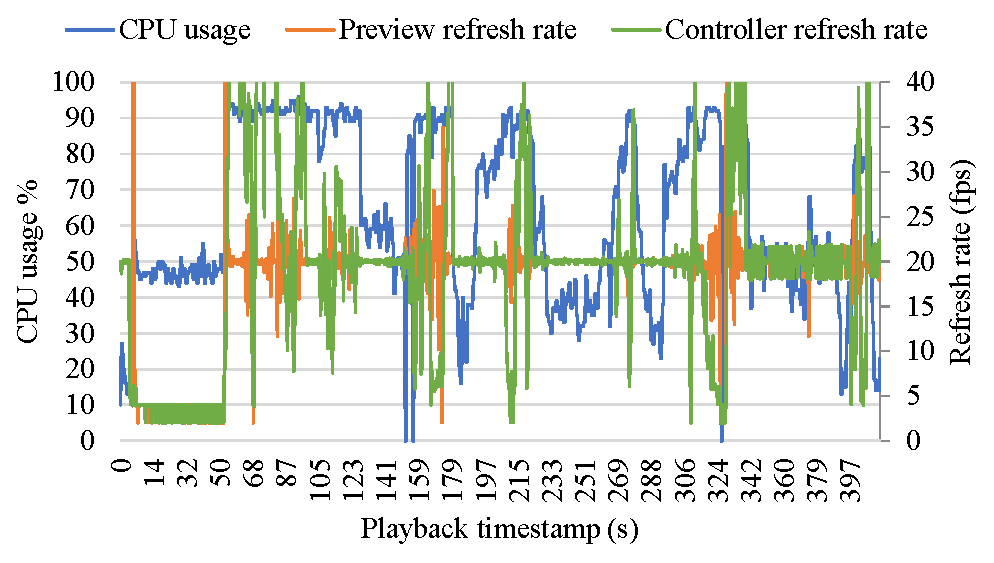
\includegraphics[width=0.8\columnwidth]{original}
  \caption{\footnotesize Performance of original Vixen execution engine}
  \label{fig:original}
\end{figure}

Further analysis using Microsoft Visual Studio's sampling profiler shows, around $24.7 \%$ of total CPU time was wasted between translation layers for generating controller commands (\texttt{GenerateCommand}), while the actual command assignment (\texttt{\_8BitEvaluator}) takes less than $0.5 \%$ of CPU time, as shown by \fref{fig:vixen_perf_original} hot path analysis. Another $23.0 \%$ CPU time was used for filter and element updates, $26.0 \%$ for preview rendering and $16.9 \%$ for the sequence editor, as shown by \fref{fig:vixen_perf_original_overview}. The CPU time used for controller updates is almost negligible.

\begin{figure}[t]
  \centering
  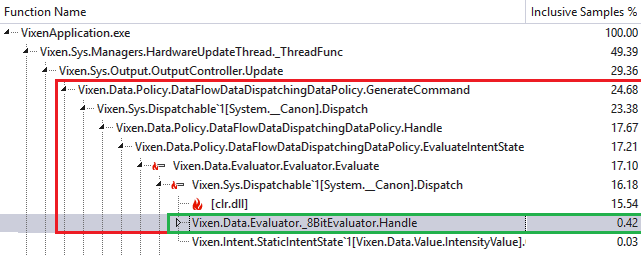
\includegraphics[width=0.85\columnwidth]{Figs/vixen_perf_original.png}
  \caption{\footnotesize Hot path analysis of Vixen update threads}
  \label{fig:vixen_perf_original}
\end{figure}

\begin{figure}[t]
  \centering
  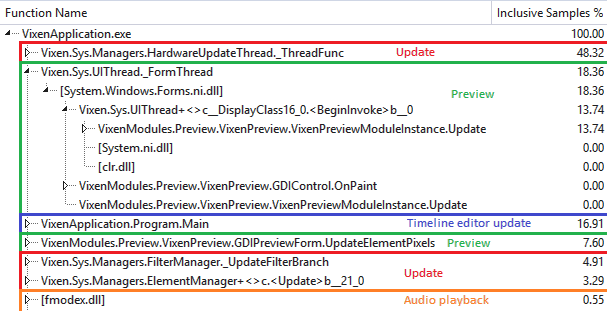
\includegraphics[width=0.85\columnwidth]{Figs/vixen_perf_original_overview.png}
  \caption{\footnotesize Hot path analysis of original Vixen application}
  \label{fig:vixen_perf_original_overview}
\end{figure}

The translation layers are used for determining the actual controller command format. There are several different command formats possible for varies controllers. For example, 8-bit, 16-bit or RGB channels. Therefore, the application need to resolve the actual types of commands for specific assignment handlers from a common command base type, which apparently very inefficient in C\#. This process is called \texttt{dispatch} in the source code, it must be minimised in order to improve performance. \wn{3}

The implementation of preview display was also very inefficient, uses only software instance management and sequential rendering. It can be improved by the utilisation of GPU through DirectX or OpenGL.

Multiple real-world lighting sequences and testing sequences were tested. They all show similar performance characteristics with unstable playback frame rate for moderately complicated lighting effects.

\section{Port to Linux}

It takes some necessary modifications for Vixen to run on Linux using mono runtime. The MonoDevelop IDE \cite{monodevelop} helps by directly supporting Microsoft Visual Studio projects. However, C/C++ projects were not supported, and pre-built dynamic runtime libraries developed using C/C++ for Microsoft Windows were also not support by mono. All code references to WPF and FMOD audio must be removed for the project to build and run.

The result Vixen application for Linux has a distorted main GUI with unreasonably long vertical window size. The sequence editor, display setup and preview would either not load or crash the entire application. Fortunately, all controller modules can be loaded and the core execution engine and controller update threads were working properly. \fref{fig:vixen_linux_main} shows some loaded controller modules and partially working GUI.

\begin{figure}[t]
  \centering
  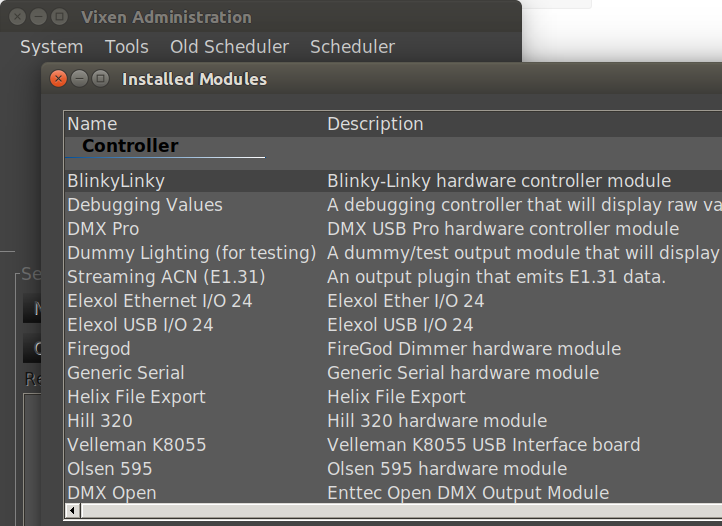
\includegraphics[width=0.8\columnwidth]{Figs/vixen_linux_controllers.png}
  \caption{\footnotesize Controller modules loaded on Linux port of Vixen application}
  \label{fig:vixen_linux_main}
\end{figure}

The intended optimised Vixen application would be command-line user interface (CUI) only with minimal essential functionality. Therefore, the broken GUI should not be an issue.

\section{Extract rendered sequence}

Instead of trying to improve the original execution engine, the performance problem may be eliminated by playing pre-rendered controller layer data frames directly to individual hardware controllers. Channel data type information can be stored separately without the need to resolve through translation layers during runtime. Element updates, Filter updates, preview and sequence editor are all necessary for playback.

Two steps are needed for this approach. Firstly, pre-render the sequence with precise frame interval, then playback the rendered data to the controllers as a separate process and perhaps on an entirely different platform.

To pre-render the sequence, two different methods are possible. A dummy controller can be used for runtime data dumping, or use a separate export engine with manual frame control independent of wall-clock time.

\section{Custom controller}
\label{sec:tcplinky}

A custom controller module (\texttt{TCPLinky}) was developed based on one of its existing controller (\texttt{BlinkyLinky}). This controller uses TCP connection to transfer display channel data, supports up to 65535 channels. A corresponding cross-platform server application that simulates a multi-channel display was also developed using C++ with Qt \cite{qt} and OpenGL \cite{shreiner2009opengl} rendering. This server application allows real-time debugging of display output without the need of a complex physical lighting system setup. Data dumping, performance and statistical analysis can also be easily achieved. \wn{4}

\fref{fig:tcplinky_server} shows a screenshot of the server application. With the help of GPU rendering through OpenGL, it consumes less than $3 \%$ of CPU time under 50 fps refresh rate, which is negligible. It can also be compiled and executed on other computers, simulates real world network connected controller scenarios.

\begin{figure}[t]
  \centering
  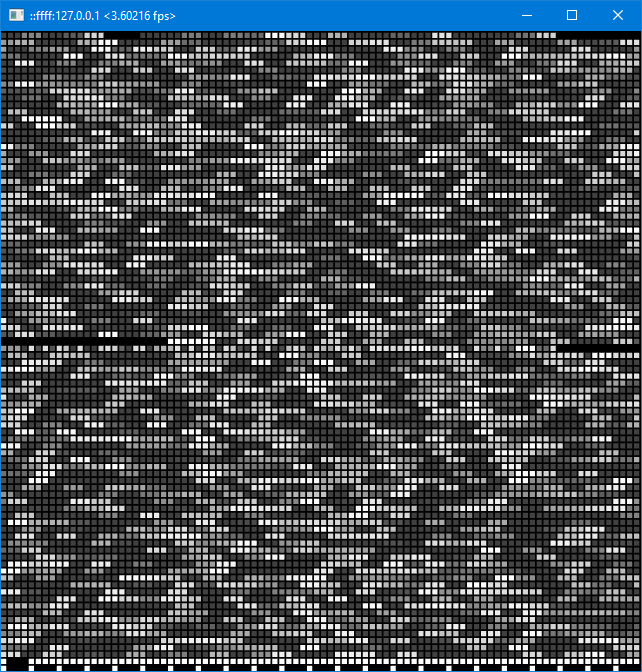
\includegraphics[width=0.6\columnwidth]{Figs/tcplinky_server.png}
  \caption{\footnotesize Screenshot of \texttt{TCPLinky} controller server application}
  \label{fig:tcplinky_server}
\end{figure}

\section{Export sequence}

Although the custom controller module is capable of dumping outputs, it can not give the indication of sequence start, end and information about other controllers. More notably, it can have unstable frame rates influenced by CPU usage. A high performance computer is needed for near prefect pre-rendering by controller dump. Therefore, the existing sequence export function from sequence editor was used instead.

The export function was originally used to convert the lighting sequence to formats recognisable by other controller specific applications. It renders the sequence using a manual timing source stepped after each frame, gives accurate constant data dump intervals. It can also write all controller channel mapping information to a separate XML file. An example XML file is shown by \lref{lst:network_xml}.

\begin{lstlisting}[float,floatplacement=ht,language=XML,label=lst:network_xml,captionpos=b,caption={\footnotesize Example controller mapping XML file}]
<?xml version="1.0" encoding="utf-8"?>
<Vixen3_Export>
  <Resolution>20</Resolution>
  <OutFile>luf2013_20ms.raw</OutFile>
  <Duration>00:04:45.8050000</Duration>
  <Network>
    <Controller>
      <Index>0</Index>
      <Name>E6804 arches L</Name>
      <StartChan>1</StartChan>
      <Channels>2048</Channels>
    </Controller>
    <Controller>
      <Index>1</Index>
      <Name>Lynx DMX</Name>
      <StartChan>2049</StartChan>
      <Channels>156</Channels>
    </Controller>
  </Network>
  <Media>
    <FilePath>example_audio.mp3</FilePath>
  </Media>
</Vixen3_Export>
\end{lstlisting}

To support the purposed optimised playback engine, audio media file path was added to the XML. The export dialog window was modified to allow custom frame resolution through text input, instead of a few pre-defined fixed values on the drop down list, as shown by \fref{fig:vixen_export}. Additional data format entries such as the ``Raw File"" for the playback engine was also added to the export wizard. This ``Raw'' format is a simple sequential concatenation of frames, where each frame compose of a 6-byte header, 2-byte channel count and followed by continuous channel data.

\begin{figure}[t]
  \centering
  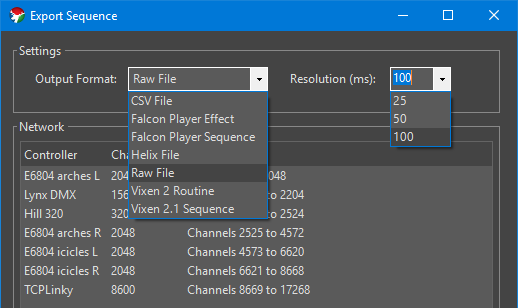
\includegraphics[width=0.75\columnwidth]{Figs/vixen_export.png}
  \caption{\footnotesize Modified Vixen export dialog window}
  \label{fig:vixen_export}
\end{figure}

\section{Source code management}

All source code related to Vixen and other programs developed in this project were managed using git version control tool \cite{git}, hosted on GitHub \cite{github} \cite{github_vixen_yz} \cite{github_project}.

Using a version control system enables history changes tracking for source code. Together with a web-based hosting service like GitHub, changes to the source code can be easily backup and synchronised on multiple devices and the cloud. The source code for official Vixen application was also hosted on GitHub \cite{github_vixen}. With GitHub's signature fork and pull request functionality, straightforward cooperation between different organisations and people can be achieved. The modifications made in this project can be therefore easily incorporated into the official Vixen application source code repository for public use.

\section{Process management}

Makefiles \cite{make} were used throughout the project for automated processing and testing. Varies text and data processing tools such as grep \cite{grep}, sed \cite{sed} and R \cite{r_project} were also used with Makefiles for automated data collection and reshaping.

\lref{lst:makefile} shows one example Makefile used for automated performance tests. Using this Makefile, following inputs will be tested sequentially with the optimised Vixen console application: raw sequence dump, \texttt{rgb24} encoded video with audio, \texttt{rgb24} video without audio, \texttt{yuv444p} encoded video without audio and \texttt{yuv420} encoded video without audio.

\chapter{Controller specific implementations}
\renewcommand{\baselinestretch}{\mystretch}
\label{chap:BG}
%\setlength{\parindent}{0pt}

To setup a reference baseline for optimal performance, sequence rendering applications dedicated to specific controllers were developed. These applications take the same sequence data file, but support only the \texttt{TCPLinky} controller developed in \sref{sec:tcplinky}. These programs were implemented as simple as possible without all intermediate layers, but still use a threading structure same as the original Vixen application.

\section{Qt2 based implementation}

A GUI application dedicated to the \texttt{TCPLinky} was developed using C++ as an optional user-friendly alternative implementation showcase. This application was developed specific to the Noah NP1380 platform listed in \sref{sec:systems}. This device is a handheld embedded device based on a 10 years old SoC chip, originally designed for educational use. \fref{fig:noah_main} shows the main interface of this device. Fortunately, this devices uses Linux system and Qt2 as GUI. Therefore, it is possible to test Vixen application on this low-end platform.

\begin{figure*}[t]
	\centering
	\subfloat[Main GUI]{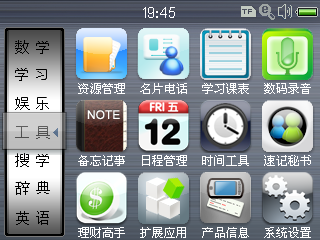
\includegraphics[width=0.45\textwidth]{Figs/noah.png}%
	\label{fig:noah_main}}
	\hfil
	\subfloat[Controller application]{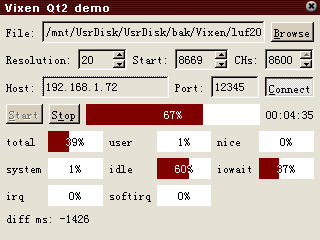
\includegraphics[width=0.45\textwidth]{Figs/vixen_noah.png}%
	\label{fig:vixen_noah}}
	\caption{Screenshot of Noah NP1380 device}
	\label{fig:noah}
\end{figure*}

\fref{fig:vixen_noah} shows a screenshot of the dedicated application. The method of performance profiling through statistic files in proc file system was also tested. These smaller progress bars at the lower half of the application shows percentages of CPU time spent on different tasks, such as user space applications, kernel mode and interrupt handling. Most of the time only less than $50 \%$ CPU time was used for this controller application, indicates even this low-end device is capable of handling thousands of lighting channels.

\section{Minimal C\# implementation}

Another minimal implementation was developed using C\#, named \texttt{VixenLinky}. Source code for controller output was ported directly from the original Vixen application. All intermediate layers and DLL loading were excluded from this implementation. With this program, the best possible performance on each platform can be measured as a reference.

The overall performance of optimised Vixen may be limited by two different factors, sequence loading performance and controller update speed. Therefore, options to unlimit the update interval of both sequence loading and controller update were added separately.

\fref{vixenlinky_rpi} shows an example of performance data gathered on the Raspberry Pi B+ platform through this program using one of real-world lighting sequences. The CPU usage peaks at $??$, while most of the time distributed around $??$ and $??$ (lower and upper quartiles).

\chapter{Playback engine}
\renewcommand{\baselinestretch}{\mystretch}
\label{chap:Playback}
%\setlength{\parindent}{0pt}

\section{Implementation and optimisation}

After verified the ability of loading and rendering the exported lighting sequence by controller dedicated implementations, the C\# code for loading exported sequence was integrated into Vixen application as a separate playback engine. Several code branches were added to switch between the original execution engine and the new playback engine. The execution engine was still used as the default engine to simplify status checking and support the sequence editor. The playback engine will only be switched to if it has started rendering sequence.

The playback engine starts by reading the exported network XML file. To simplify the process, XML object serialiser was used to interpret the XML file to a similarly structured object for later access. The information from XML will be used to determine controller channel mapping, update interval and optional audio media file. To further reduce overhead, the controller names will be looked up and converted to their unique ID (GUID) for later lookup. The optional audio media file was supported by utilising the same audio media functions from original execution engine.

All preview, element and filter updates were skipped in the playback engine. The translation layers were skipped, since the sequence data is already specific to the controllers. However, in order to match the existing interface of controller modules, the sequence data still need to be copied again to specific command types, incurred some unnecessary overhead.

The structure of update management was also changed. Previously, the application updates the channel data buffer from any controller update request, which requires the use of mutex to lock data access between controller threads. With a configuration of multiple controllers, potential lock contention of the mutex can also incur some overhead. Another thread dedicated to sequence loading was add to the playback engine to address this issue, similar to the structure of controller specific implementations. In this way, only the sequence loading thread may update the channel data buffer, removed the need of mutex locker.

One major drawback of using the playback engine is that the data dump cannot be mapped back to element states yet. Therefore, editing the sequence using the built-in editor and the preview output were not supported.

\section{Integration}

A simple control dialog was added as a menu entry for the preview engine, as shown by \fref{fig:vixen_playback}. More complex and user-friendly UI design is possible, however, due to limited time constraint this control dialog should be sufficient for this project and proof of concept.

\begin{figure}[t]
  \centering
  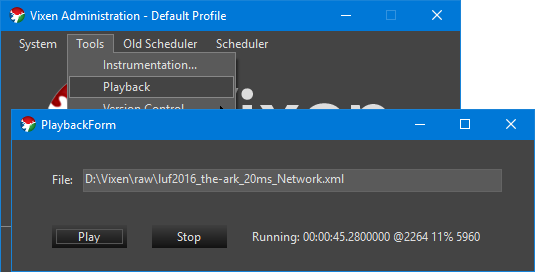
\includegraphics[width=0.8\columnwidth]{Figs/vixen_playback.png}
  \caption{\footnotesize Screenshot of the playback engine controller}
  \label{fig:vixen_playback}
\end{figure}

The playback control was also integrated with built-in schedulers. It can therefore be scheduled to execute multiple times at specific time, possibly with schedules using the original execution engine. The new playback engine does not need additional pre-process for show schedules, can be directly started within seconds.

\section{Performance}

\fref{fig:playback} shows the performance of the playback engine using a ``Raw'' sequence dump. At the first and the last few seconds, the playback engine stopped, the original execution engine was used instead during idle state. However, the execution engine still uses around $30 \%$ of CPU time during idle. But as soon as playback started, CPU usages drops to around $6 \%$ with stable refresh frame rates.

\begin{figure}[t]
  \centering
  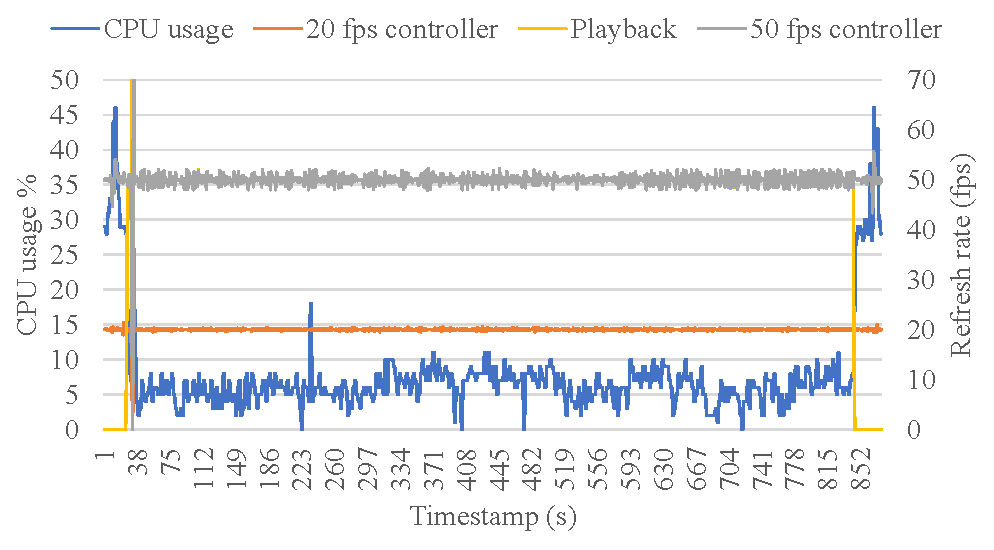
\includegraphics[width=0.8\columnwidth]{playback}
  \caption{\footnotesize Performance of new playback engine}
  \label{fig:playback}
\end{figure}

\chapter{Console application}
\renewcommand{\baselinestretch}{\mystretch}
\label{chap:Console}
%\setlength{\parindent}{0pt}

\section{Implementation}

A Command-line User Interface (CUI) version of Vixen, named \texttt{VixenConsole}, was implemented for Linux based platforms. It is easier to operate and manage a CUI based program through remote connection instead of a distorted partially functional GUI application. \cref{chap:Guide} listed the detailed usage description of \texttt{VixenConsole}.

The original core codebase from \texttt{Vixen.dll} was used in this program with some necessary modifications. Instead of full initialisation from Vixen GUI application, only minimal initialisation of output controllers will be done from \texttt{VixenConsole} to reduce overheads. In this way, the code for the playback engine, module and data loading is still shared with the Vixen GUI application, including future improvements and patches.

\texttt{VixenConsole} reads configurations from the same location as Vixen application, the \texttt{Vixen 3} folder from user home directory. All configurations are stored as XML files, exported directly from settings object using XML serialiser. The ability to list available controllers and their configurations were added to \texttt{VixenConsole}. However, configuration modification was not yet possible from \texttt{VixenConsole}, due to the complexity of supporting every types of configuration fields within the project time constraint. To create or modify the configuration, the Vixen GUI application can be used from a computer running Microsoft Windows. Editing the XML configuration files directly using text editors is also possible.

\section{Loading performance}

On an embedded platform with limited computation power, the loading time of \texttt{VixenConsole} and all controller modules can take a significant time. The implemented \texttt{tidy} operation can reduce a small portion of the loading time, by remove unused settings for elements and filters. It also reduces the size of XML settings file.

However, it still takes more than 2 minutes from starting \texttt{VixenConsole} to rendering on the Noah NP1380 platform. This loading time is for the mono runtime to preform some necessary tasks such as dynamic recompile, thus unavoidable.

\section{Execution performance}

\fref{fig:raw-seq-p-c} compares the performance between \texttt{VixenLinky} and \texttt{VixenConsole} on multiple platforms. The performance comparison was done by unlimit the playback and controller refresh rate separately using both \texttt{VixenLinky} and \texttt{VixenConsole} applications, a total number of 4 tests on each of the platforms. The refresh rate data over the entire sequence time then summarised to a five-number summary representation, i.e. sample minimum, lower quartile, median, upper quartile and sample maximum. The mean values were also plotted as lines for comparison. The refresh rate axis is log scale, to focus on the lower performance figures over all platforms.

\begin{figure}[t]
  \centering
  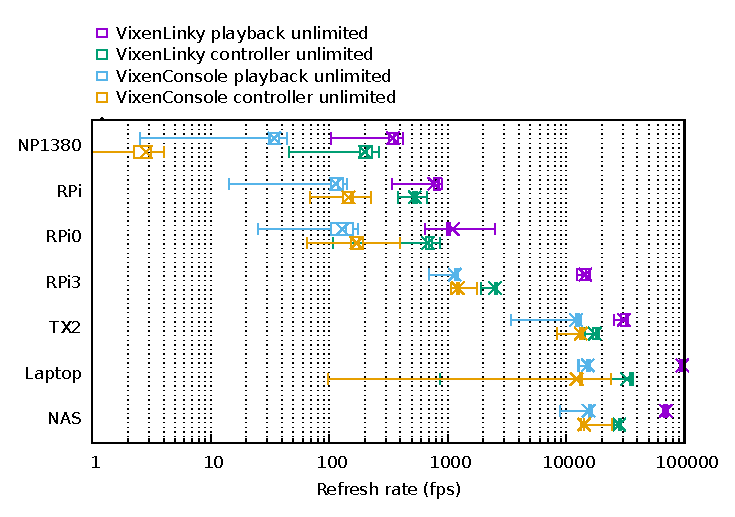
\includegraphics[width=0.9\textwidth]{Figs/raw-seq-p-c.eps}
  \caption{\footnotesize Performance comparison between \texttt{VixenLinky} and \texttt{VixenConsole}}
  \label{fig:raw-seq-p-c}
\end{figure}

By separating playback and controller update tests, the two major performance limitation factors of file IO and processing power can be separately tested.

The figure shows, \texttt{VixenConsole} runs a few times slower than the minimal implementation \texttt{VixenLinky}. On NP1380, the controller refresh rate drops below 10 fps, unusable for a 50 fps sequence. It still performs adequately on Raspberry Pi B+, both the maximum possible playback and controller refresh rate were significantly higher than 50 fps.

The mono profiler was used in an attempt to determine the most time consuming code segment on Raspberry Pi. However, it was not particularly useful. As shown by \lref{lst:mono_sample}, the information given by the profiler does not give notable highlight for performance optimisation opportunity. Apart from unhelpful unknown methods, the thread sleeping method, file reading methods and update methods are all just as expected. Some overheads from copying command arrays do show up on the summary as array coping functions, but they are unavoidable for controller module interface compatibility.

\begin{lstlisting}[float,floatplacement=ht,language=,label=lst:mono_sample,captionpos=b,caption={\footnotesize Summary of time spent in each method collected by mono profiler}]
Method call summary
Total(ms) Self(ms)      Calls Method name
  796551   796551      19237 (wrapper managed-to-native) System.Threading.Thread:SleepInternal (int)
  516874   516771       3785 (wrapper managed-to-native) System.IO.InotifyWatcher:ReadFromFD (intptr,byte[],intptr)
 1646781   412701      58603 unknown method 0xffffffffb2b3bb88
33649154   137328      58651 VixenModules.Output.TCPLinky.TCPLinky:UpdateState (int,Vixen.Commands.ICommand[])
   94269    57976      18249 Vixen.Sys.Playback:ReadFrame ()
   37151    37151     188864 (wrapper managed-to-native) object:__icall_wrapper_ves_icall_array_new_specific (intptr,int)
   31689    31689      47264 (wrapper managed-to-native) System.IO.MonoIO:Read (intptr,byte[],int,int,System.IO.MonoIOError&)
   27701    27701     123629 (wrapper managed-to-native) System.Array:FastCopy (System.Array,int,System.Array,int,int)
15553611    21874       8829 unknown method 0x102b29cc0
 9115056    20593      58659 unknown method 0xffffffffb2b38660
   22427     9027     387111 System.Diagnostics.Stopwatch:get_ElapsedMilliseconds ()
   13421     8374     387116 System.Diagnostics.Stopwatch:get_ElapsedTicks ()
43869866     7960      58635 Vixen.Sys.Output.OutputController:Update ()
    7604     7604     565017 (wrapper managed-to-native) System.Diagnostics.Stopwatch:GetTimestamp ()
    6167     6167       3020 (wrapper managed-to-native) System.Runtime.CompilerServices.RuntimeHelpers:SufficientExecutionStack ()
 4779217     5777       8845 unknown method 0x102263018
 2615069     4814      17466 unknown method 0x102264df8
    4509     4509       8821 (wrapper managed-to-native) System.Net.Sockets.Socket:Send_internal (intptr,byte[],int,int,System.Net.Sockets.SocketFlags,int&,bool)
\end{lstlisting}

\chapter{Video data format}
\renewcommand{\baselinestretch}{\mystretch}
\label{chap:Video}
%\setlength{\parindent}{0pt}

With the implementation of \texttt{VixenConsole}, the process of designing and pre-rendering (exporting) the sequence on Vixen application then playback later using \texttt{VixenConsole} became very similar to the process of video editing and playback. Therefore, it may be beneficial to add support for video sequence format.

\section{Implementation}

The open source \texttt{ffmpeg} framework \cite{ffmpeg} was used for video processing. The open source nature ensures up-to-date version of \texttt{ffmpeg} is available on all testing platforms.

The \texttt{ffmpeg} framework uses the C programming language for its API. The complicity of different data structures used by \texttt{ffmpeg} results in no up-to-date C\# wrapper API available for use directly. Therefore, an intermediate wrapper layer between Vixen and \texttt{ffmpeg} was developed to encapsulate all complex \texttt{ffmpeg} routines using C.

The development of video integration was separated into multiple steps. Firstly, several C programs were developed to test individual video processing functions including video encoding, video decoding, stream muxing and metadata retrieve. Afterwards, working code segments were combined into a dynamic library, with a simplified API suitable for C\#. A C\# wrapper class was then developed using the \texttt{InterOp} service \cite{interop}, together with another C\# program for testing video encoding and decoding. After all these small testing programs had been confirmed working, the C\# wrapper was finally integrated into Vixen with the playback engine. The playback engine checks for input file extension to determine whether to load the file as exported ``Raw'' sequence or video file.

To ensure lossless transcoding from the ``Raw'' sequence to video stream, the transcoding programs were tested by encoding example sequences to video then decoded back to another sequence. The two sequences were then compared for any difference, using the GNU \texttt{diff} tool \cite{diff}. Makefile was used for automated compiling and testing.

To minimise number of files needed for playback, the optional audio file was muxed together with the video stream, and the network configuration XML file was stored directly as string literal in video metadata field ``comment'', as shown by \fref{fig:video-info}.

\begin{figure}[t]
  \centering
  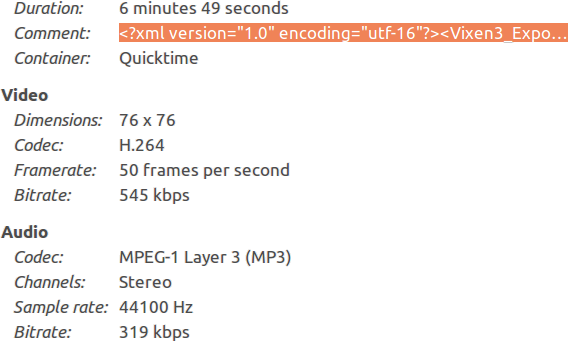
\includegraphics[width=0.7\textwidth]{Figs/video_info.png}
  \caption{\footnotesize Media information of an example video sequence}
  \label{fig:video-info}
\end{figure}

In the playback engine, video frames will be transformed to controller data frames for rendering. However, the existing audio rendering engine \texttt{FMOD} from Vixen only supports media file playback. The required functionality of playing decoded data frames was not available from its C\# API. To resolve this issue, C code for operating a newer version of \texttt{FMOD} was added to the wrapper library. The playback engine transfers the decoded audio frame back to the wrapper library for audio playback.

\section{Benefits and limitations}

The first noticeable benefit was reduction in sequence file size. The ``Raw'' sequence format was implemented without any compression algorithm, always has a size linear to total sequence time and channel count. The video formats reduced the sequence size to around $\frac{1}{10}$ of the ``Raw'' sequence. \tref{tbl:size} compares file sizes in different formats of the same example sequence.

\begin{table}[t]
  \centering
  \begin{tabular}{l|l|l}
    \hline
    \textbf{Type} & \textbf{Sequence size} & \textbf{With audio} \\
    \hline
    Editable sequence                     & 8.88 MiB  & 24.4 MiB  \\ \hline
    50 fps exported \texttt{Raw} sequence & 337 MiB   & 352 MiB   \\ \hline
    50 fps \texttt{rgb24} encoded video   & 26.6 MiB  & 42.5 MiB  \\ \hline
    50 fps \texttt{yuv444p} encoded video & 26.6 MiB  & 42.5 MiB  \\ \hline
    50 fps \texttt{yuv420p} encoded video & 18.2 MiB  & 34.1 MiB  \\ \hline
  \end{tabular}
  \caption{\footnotesize File size comparison of different formats}
  \label{tbl:size}
\end{table}

Using the video format, the exported sequence, audio and configuration information are combined into a single file. This reduction of file count can sometimes simplify the management and sharing of multiple sequences.

The \texttt{yuv420p} encoded video listed in \tref{tbl:size} were transcoded from the \texttt{rgb24} encoded video using the \texttt{ffmpeg} command-line tool. It is possible to add support for multiple video formats as options to the developed video library to directly transcode from ``Raw"" sequence to other video formats. However, this can make the encoding process over complicated. Instead, other dedicated video transcoding tools can be used for the same task. The decoding routine used in playback engine was designed to support any video encoding format, by converting the video frames to \texttt{rgb24} format internally. This is another benefit of using a video file. All tools developed for general purpose video processing and editing can also be used for the exported sequences.

With these sophisticated video compressing algorithms, a drop of the sequence loading speed was expected. Fortunately, the \texttt{ffmpeg} library is capable of utilising media acceleration features to speed up video decoding, such as SIMD instructions and dedicated video decoding hardware. However, a small resolution video, such as the $76 \times 76$ video from \fref{fig:video-info}, is more than capable of supporting thousands of controller channels. It may not leverage the full advantage of dedicated high resolution hardware video decoding accelerators.

Within the 3 formats tested, \texttt{yuv420p} probably is the most common video encoding format currently. It is also more commonly supported by hardware video accelerators. However, \texttt{yuv420p} is not capable to store channel data losslessly with the same frame resolution. It is more suitable for storing realistic videos, where sudden colour changes between pixels are uncritical and not common. Colour degrade and cross-talk between channels are unavoidable with the \texttt{yuv420p} encoding format.

\cmt{Varies encoding, formats, quality factor... Insert data table \wn{16}}

\chapter{User Guide}
\renewcommand{\baselinestretch}{\mystretch}
\label{chap:Video}
%\setlength{\parindent}{0pt}

\cmt{\url{http://www.imperial.ac.uk/electrical-engineering/internal/current-students-course-handbook/msc-individual-research-project/writing-the-report-}}

\chapter{Conclusion}
\renewcommand{\baselinestretch}{\mystretch}
\label{chap:Conclusion}
%\setlength{\parindent}{0pt}

\PARstart{T}{he} runtime performance of Vixen lighting control application was \ca{substantially} improved, by changing the data preparation process and developing a new simplified playback engine. \ca{With the new playback engine,} embedded platforms are now able to easily handle sophisticated lighting sequences with thousands of controller channels.

A new CUI application with the new playback engine was developed specifically for embedded platforms to simplify control and management operations. Using an embedded device instead of a powerful computer to control the lighting controllers also gives greater flexibility with reduced power consumption \ca{and cost}.

Sequence \cb{exporting} and playback of video \cb{formatted sequences} were implemented. Commonly available video processing, editing and analysing tools can be used together with the playback engine for more functionality and flexibility. The video format together with audio stream muxing and metadata configuration support also helps with data management and sharing.

\section{Limitations}

Although the performance improvement was huge, the \texttt{VixenConsole} application was still unavoidably slower than controller \ca{specific} implementations, due to its generic modular design.

The video sequences generally have extremely small frame resolution compared to modern videos and movies. The optimal encoding format requirements for sequences are also different from realistic videos. Therefore, the Vixen application may not benefit much from common video \ca{formats and} processing tools \ca{targeted at realistic videos for post editing \cb{purposes}}.

Although the CUI application gives easier controllability with performance improvements, it is not as intuitive and user-friendly as a GUI application. For users without previous experiences of using CUI applications, it can be very confusing to work with.

\section{Future works}

Some code segments, such as the playback engine control form (\fref{fig:vixen_playback}), can be improved. These code segments were implemented only with proof-of-concept level of details. More extensive exception checks and user friendly additional functionalities are needed.

The integration between original execution engine and the new playback engine can be improved. Currently, the playback engine takes priority over the execution engine, which might cause undesired behaviour under certain circumstances. The execution engines should also be switched off during idle to further reduce CPU usage.

Support for element back-mapping and preview display was not implemented for the playback engine yet. It may require extraction of mapping configurations during export.

The video channel mapping can be more intuitive. For example, map controller channels using the preview layout design. In this way, the sequence can be directly previewed and edited using existing multimedia software.


%%%%%%%%%%%%%%%%%%%%%%
% The reference list.%
%%%%%%%%%%%%%%%%%%%%%%

\renewcommand{\baselinestretch}{1}

% Note: put the bib style and bib file you use here.
\bibliographystyle{IEEEtran}
\bibliography{IEEEabrv,references}

%%%%%%%%%%%%%%%%%%%%%%%%%%%%%
% The end of reference list.%
%%%%%%%%%%%%%%%%%%%%%%%%%%%%% 

\fancyhead[RE]{\emph{References}}

\appendix
\renewcommand{\baselinestretch}{1.5}
\chapter{Makefile for automated tests}
\label{App:tests}

\begin{lstfloat}
\begin{lstlisting}[language=make,label=lst:makefile,captionpos=b,caption={\footnotesize Makefile used for automated performance tests}]
SEQ	= ~/Vixen/luf2016_the-ark_20ms_Network.xml
VA	= ~/Vixen/2016.rgb24.audio.test_enc.mp4
V	= ~/Vixen/2016.rgb24.test_enc.mp4
VYUV	= ~/Vixen/2016.yuv444p.test_enc.mp4
V420	= ~/Vixen/2016.yuv420p.test_enc.mp4

CONSOLE	= MONO_IOMAP=all mono VixenConsole.exe
PERF	= 500
PERF_PB	= 100

.PHONY: all
all: raw seq va v vyuv v420

.PHONY: seq va v vyuv v420
seq: seq-normal seq-playback seq-controller
va: va-normal va-playback va-controller
v: v-normal v-playback v-controller
vyuv: vyuv-normal vyuv-playback vyuv-controller
v420: v420-normal v420-playback v420-controller

seq-normal seq-playback seq-controller: $(SEQ)
va-normal va-playback va-controller: $(VA)
v-normal v-playback v-controller: $(V)
vyuv-normal vyuv-playback vyuv-controller: $(VYUV)
v420-normal v420-playback v420-controller: $(V420)

%-normal:
	mkdir -p prof; $(CONSOLE) -p $(PERF) start $<; mv prof $@
%-playback:
	mkdir -p prof; $(CONSOLE) -p $(PERF_PB) -u playback start $<; mv prof $@
%-controller:
	mkdir -p prof; $(CONSOLE) -p $(PERF) -u controller start $<; mv prof $@
\end{lstlisting}
\end{lstfloat}

\iffalse
\lref{lst:makefile} shows one Makefile used for video transcoding and PSNR testing.

\begin{lstlisting}[float,floatplacement=ht,language=XML,label=lst:makefile,captionpos=b,caption={\footnotesize Makefile used for automated video transcoding}]
INPUT	?= $(wildcard *raw.mp4)
AUDIO	?= $(wildcard *audio.mp3)
OUTPUT	:= yuv444p-0.mp4 yuv444p-6.mp4 yuv444p-12.mp4 yuv420p-0.mp4
OUTPUT	+= rgb24-0.mp4 rgb24-6.mp4 rgb24-12.mp4 rgb24-24.mp4 rgb24-0-audio.mp4
ROOT	:= $(dir $(realpath $(lastword $(MAKEFILE_LIST))))

all: $(OUTPUT)
psnr: $(OUTPUT:%=psnr-%)

.SECONDARY:
.DELETE_ON_ERROR:
yuv420p-%.mp4: $(INPUT)
	ffmpeg -i "$<" -crf $* -codec:v libx264 -pix_fmt yuv420p -y "$@"
yuv444p-%.mp4: $(INPUT)
	ffmpeg -i "$<" -crf $* -codec:v libx264 -pix_fmt yuv444p -y "$@"
rgb24-%.mp4: $(INPUT)
	ffmpeg -i "$<" -crf $* -codec:v libx264rgb -pix_fmt rgb24 -y "$@"
rgb24-%-audio.mp4: $(INPUT) $(AUDIO)
	ffmpeg -i "$(INPUT)" -i $(AUDIO) -c:v copy -c:a copy "$@"
psnr-%: $(ROOT)psnr.sh % $(INPUT)
	$^ 2>&1 | tail -n 1
\end{lstlisting}
\fi


%%%%%%%%%%%%%%%%%%%%%%%%%%%%%%
% The end of a LaTeX document
\end{document}

%%%%%%%%%%The END%%%%%%%%%%%%%%%%%%%%
